\documentclass[11pt,a4paper]{article}
\usepackage[hyperref]{acl2023}
\usepackage{graphicx}
\title{Behavior Simulation and Content Simulation}
\author{Yash Kumar, Vivek Yadav, Vishal Das \\
  Department of Computer Science and Technology \\
  Delhi Technological University, Delhi, India \\
  {\tt \{yashkumar\_co21a8\_34, vivekyadav\_co21a8\_30, vishaldas\_co21a8\_24\}@dtu.ac.in}}

\date{April 04, 2024}

\begin{document}
\maketitle

\begin{abstract}
This document provides an overview of the data science challenge on "Behavior Simulation and Content Simulation." The challenge focuses on estimating user engagement on social media content and creating content that aligns with key performance indicators (KPIs).
\end{abstract}

\section{Introduction}
The goal of the challenge is to address the complexities of user behavior and engagement on social media platforms, particularly Twitter. The dataset comprises sampled tweets from enterprise accounts over the past five years, including metrics such as likes, retweets, and comments.

\section{Problem Description}
The problem statement outlines the communication process and user engagement on social media. Our task is to analyze the provided dataset and develop models that can predict user engagement based on various features.

\section{Phase 1: Exploratory Data Analysis}
During this phase, we will clean and preprocess the dataset. Exploratory Data Analysis (EDA) techniques will be applied to understand data characteristics, identify outliers, and generate insights for subsequent modeling. Cleaning methods will include text normalization, punctuation removal, and other necessary steps.

\subsection{Data Cleaning}
We will normalize text data, remove unwanted characters, and prepare the dataset for further analysis. We will also be extracting hashtags present in the tweets and use it for fruther analysis.

\subsection{Exploratory Data Analysis}
\begin{figure}
    \centering
    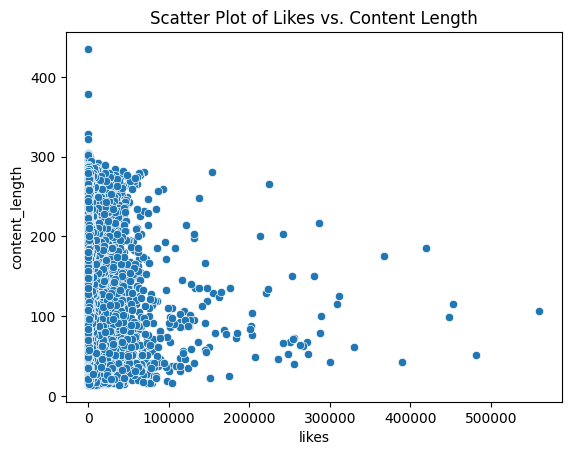
\includegraphics[width=0.5\linewidth]{likes_vs_content.png}
    \caption{Like vs Content Length Scatterplot}
    \label{fig:scatter1}
\end{figure}
The analysis of the graph in Figure \ref{fig:scatter1} indicates that the content\_length alone does not serve as a reliable predictor for likes. This is evident from the substantial variance in likes observed at content\_length = 0. However, the presence of other favorable factors can enhance the predictability. In such cases, having a content\_length around the median value tends to be beneficial.
\begin{figure}
    \centering
    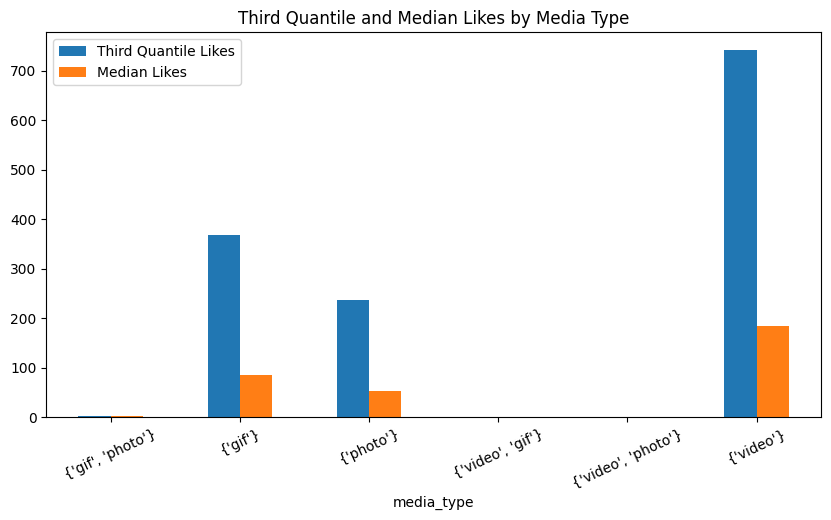
\includegraphics[width=0.5\linewidth]{likes_by_media_type.png}
    \caption{Enter Likes by media type}
    \label{fig:likes_media}
\end{figure}

From the analysis presented in Figure \ref{fig:likes_media}, it is evident that the ‘video’ media type garners approximately twice the number of likes compared to the ‘photo’ media type. This suggests a higher level of user engagement with video content on the platform.

\begin{figure}
    \centering
    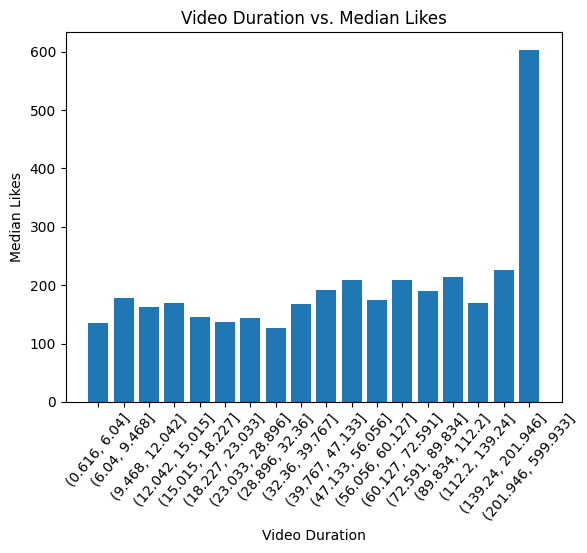
\includegraphics[width=0.5\linewidth]{duration_median.png}
    \caption{Video duration and median likes}
    \label{fig:duration_median}
\end{figure}

An analysis of bar graph \ref{fig:duration_median} reveals a discernible correlation between video duration and their corresponding median likes. Most bars are of moderate height, indicating a moderate number of median likes for those respective video durations. However, there is a noticeable spike in the last bar on the right, indicating a significantly higher number of median likes for videos within that particular duration segment. This pattern suggests a potential relationship between the two variables.

In bar graph in figure \ref{fig:median-likes-vs-hashtags}, our analysis underscores a significant correlation between the popularity and contemporaneity of hashtags and the median likes received by tweets incorporating those hashtags. The dataset, comprising hashtags utilized by at least four distinct brands in their tweets, reveals a discernible pattern: an augmentation in median likes is concomitant with the increased prevalence of the hashtag. Furthermore, temporal relevance emerges as a pivotal factor; hashtags echoing ongoing events or prevailing trends tend to amass a higher number of likes. This observation is instrumental in delineating the dynamics of user engagement on social media platforms and can be integral in strategising content dissemination to optimize user interaction.

\begin{figure}
    \centering
    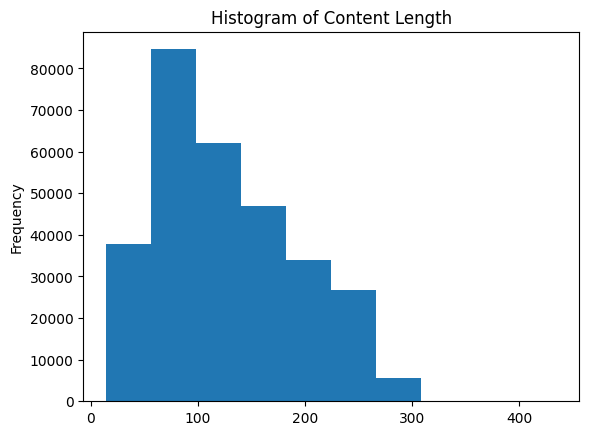
\includegraphics[width=0.5\linewidth]{content_len_histogram.png}
    \caption{Frequency vs Content-Length}
    \label{fig:enter-label}
\end{figure}

\begin{figure}
    \centering
    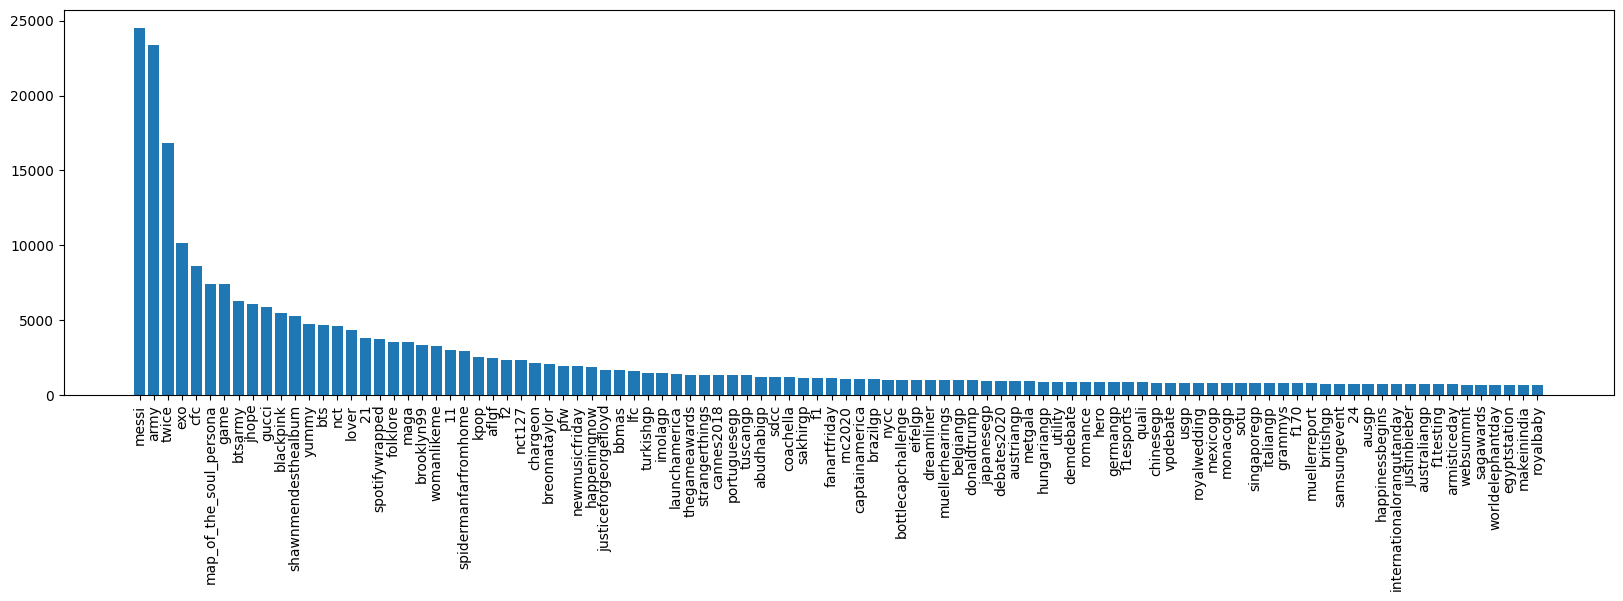
\includegraphics[width=1.0\linewidth]{median_likes_vs_hashtags.png}
    \caption{Median Likes vs Popular Hashtags}
    \label{fig:median-likes-vs-hashtags}
\end{figure}

\end{document}
